% Compile with Tectonic or XeLaTeX (twice) from this directory.
\documentclass[10pt,a4paper]{article}
\usepackage[left=20mm,right=20mm,top=30mm,bottom=22mm,headheight=28pt,headsep=12pt]{geometry}
\usepackage[T1]{fontenc}
\usepackage{lmodern}
\usepackage{amsmath,amssymb,booktabs,tabularx,array,graphicx}
\usepackage{fancyhdr,microtype,enumitem,caption,float,placeins}
\usepackage[hidelinks]{hyperref}
\usepackage{bookmark,lastpage}
\setlength{\parindent}{0pt}
\setlength{\parskip}{5pt}
\setlength{\emergencystretch}{2em}
\renewcommand{\arraystretch}{1.17}
\setlist{nosep,leftmargin=1.5em}
\captionsetup{font=small,labelfont=bf,labelsep=period}
\setcounter{tocdepth}{2}
\graphicspath{{figures/}}
\pagestyle{fancy}
\fancyhf{}
\fancyhead[L]{\small\ttfamily HO CHI MINH CITY UNIVERSITY OF TECHNOLOGY\\
FACULTY OF COMPUTER SCIENCE AND ENGINEERING}
\fancyfoot[L]{\scriptsize\ttfamily CO3133 -- HK261 \quad Team G-09}
\fancyfoot[R]{\scriptsize\ttfamily \thepage}
\renewcommand{\headrulewidth}{.4pt}
\renewcommand{\footrulewidth}{.4pt}
\hypersetup{pdftitle={Fashion-MNIST Image Classification: A Comparison of Five Neural Models},
pdfauthor={Nguyen Vu Long; Le Phuoc Vu; Nguyen Hoang Quoc},
pdfsubject={CO3133 Assignment 1, complete report}}
\makeatletter
\newcommand{\tabledata}[1]{\@@input #1 }
\makeatother
\newcommand{\UpperErrors}{532}
\newcommand{\UpperErrorPercent}{66.0}
\newcommand{\SharedErrors}{389}
\newcommand{\MlpOnly}{360}
\newcommand{\LstmOnly}{358}

\begin{document}
\hypersetup{pageanchor=false}
\begin{titlepage}
\centering
{\large VIETNAM NATIONAL UNIVERSITY HO CHI MINH CITY\par}
\vspace{4pt}
{\large\bfseries HO CHI MINH CITY UNIVERSITY OF TECHNOLOGY\par}
\vspace{4pt}
{\normalsize FACULTY OF COMPUTER SCIENCE AND ENGINEERING\par}
\vspace{1.2cm}

\includegraphics[width=2.7cm]{hcmut-logo.png}\par
\vspace{1.1cm}
{\large Deep Learning and Its Applications (CO3133)\par}
\vspace{.6cm}
{\Large\bfseries ASSIGNMENT 1\par}
\vspace{.6cm}
{\Huge\bfseries Fashion-MNIST\par}
\vspace{.2cm}
{\LARGE\bfseries Image Classification\par}
\vspace{.5cm}
{\large A Comparison of Five Neural Models\par}
\vspace{1cm}
\begin{tabular}{ll}
\textbf{Lecturer} & Le Thanh Sach\\
\textbf{Class / Team} & CC01 / G-09\\[9pt]
\textbf{Student} & \textbf{Student ID}\\
Nguyen Vu Long & 2352696\\
Le Phuoc Vu & 2353341\\
Nguyen Hoang Quoc & 2353027\\
\end{tabular}
\vfill
{Ho Chi Minh City, October 2026\par}
\end{titlepage}
\pagenumbering{roman}
\hypersetup{pageanchor=true}
\phantomsection
\section*{Abstract}
\addcontentsline{toc}{section}{Abstract}
This report compares five neural network configurations for Fashion-MNIST image
classification: a Linear classifier, a multilayer perceptron (MLP), a convolutional
neural network (CNN), a row-sequence LSTM and a patch-based Transformer.
The models receive the same pixels, arranged as vectors, image grids, rows or
patches. The study examines how these choices relate to predictive quality,
training behavior and computational cost.

The official training data is divided into 54,000 training and 6,000 validation
images using a stratified split with seed 42. The official test set contains
10,000 images. Normalization uses statistics from the training partition only.
All five models use Adam with a learning rate of 0.001, batches of 128 and ten
epochs, without data augmentation. The checkpoint with the lowest validation
loss is evaluated on the test set.

The CNN achieves the highest test accuracy, 91.94\%, and macro-F1, 0.9189.
MLP and LSTM obtain 88.50\% and 88.48\% accuracy, followed by Transformer at
85.55\% and Linear at 84.26\%. The CNN makes 806 errors, compared with
1,150 for the MLP. It also has the most parameters, at 421,642. Under the recorded
GTX 1660 SUPER inference measurement, the MLP takes 0.247 milliseconds per
128-image forward batch and the CNN takes 1.074 milliseconds.

Class-level analysis shows that upper-body garments remain the main difficulty.
The CNN correctly identifies 71.8\% of Shirt images, compared with 98.8\% of
Trouser images. Its mistakes often occur between Shirt, T-shirt/top, Pullover
and Coat. These errors are consistent with the similar silhouettes observed
in the training data, although that observation alone does not establish why
an individual prediction failed.

The results favor the implemented CNN for accuracy and show the MLP as a useful
lower-cost alternative in the recorded batch timing. Conclusions are limited
to one seed and the tested configurations. Model capacity differs, training
hardware is not shared across all five runs, and the study does not estimate
variation across repeated training runs.

\vspace{8pt}
\textbf{Keywords:} Fashion-MNIST; image classification; CNN; LSTM; Transformer;
model comparison.

\clearpage
\begingroup
\setlength{\parskip}{0pt}
\tableofcontents
\endgroup
\clearpage
\pagenumbering{arabic}
\section{Introduction}
\label{sec:introduction}
\subsection{Background and motivation}
Image classification assigns a category to an image. For a product catalogue,
this could help organize new items into clothing and accessory groups.
Reliable classification depends on more than the model: the data split,
preprocessing and evaluation procedure also affect how a result should be
interpreted.

Fashion-MNIST provides a manageable setting for studying this process
\cite{fresh_fashion}. Its small grayscale images make it practical to train
several models, while visually similar categories create a useful recognition
challenge. A shirt and a pullover, for example, may have similar outlines even
though they belong to different labels.

Different architectures use image information in different ways. A Linear
classifier combines pixel values directly. An MLP learns nonlinear combinations
of pixels. A CNN learns local spatial patterns, an LSTM reads an ordered sequence
of rows, and a Transformer combines information across image patches.
Comparing these approaches helps explain what each design contributes in a
small, controlled experiment.

\subsection{Problem statement}
The task is supervised, single-label classification into ten categories.
A raw image is $X\in\{0,\ldots,255\}^{28\times28}$ and its label is
$y\in\{0,\ldots,9\}$. After preprocessing $T$, a model with parameters $\theta$
produces ten scores:
\[
f_\theta(T(X))=z\in\mathbb{R}^{10},
\qquad \hat y=\arg\max_{k\in\{0,\ldots,9\}}z_k.
\]
The prediction describes the complete image. The study does not locate objects
within an image or assign several labels to one image.

The main question is how the five implemented configurations compare when they
use the same training examples, normalization and epoch budget. We examine both
overall performance and the types of mistakes hidden by an aggregate score.

\subsection{Objectives and scope}
The project has four objectives:
\begin{enumerate}
\item Inspect the dataset and establish a reproducible preprocessing and split protocol.
\item Implement and compare Linear, MLP, CNN, LSTM and Transformer classifiers.
\item Evaluate accuracy, macro-F1, learning behavior and class-specific errors.
\item Relate predictive quality to parameter count and documented runtime measurements.
\end{enumerate}

The experiments use Fashion-MNIST only, with no pretrained weights, external
training data or augmentation. Each model is trained once using seed 42 and ten
epochs. The comparison concerns these particular configurations; architecture,
parameter count and computation are not independently controlled.

\subsection{Report approach}
Section~2 describes the data, exploratory findings and preprocessing.
Section~3 explains the models and the common training procedure.
Section~4 compares the saved results and runtime measurements.
Section~5 examines class-level and image-level errors.
Sections~6 and 7 discuss the limitations and conclusions.
The appendices provide the numerical class results, additional confusion matrices
and reproduction instructions.

The analysis uses the existing completed runs. Their saved predictions are used
to recompute accuracy, class scores and confusion counts. Validation selects
the checkpoint; the reported test results are kept separate from that selection.

\clearpage
\section{Dataset and Exploratory Analysis}
\label{sec:dataset}
\subsection{Dataset and partitioning}
Fashion-MNIST contains 60,000 official training images and 10,000 official test
images \cite{fresh_fashion,dataset_repository}. Each image has $28\times28$
grayscale pixels, with integer intensities from 0 to 255. There are ten labels,
listed in Table~\ref{tab:labels}.

\begin{table}[H]\centering
\caption{Fashion-MNIST labels used throughout the report.}\label{tab:labels}
\begin{tabular}{clcl}\toprule
Label & Category & Label & Category\\\midrule
0 & T-shirt/top & 5 & Sandal\\
1 & Trouser & 6 & Shirt\\
2 & Pullover & 7 & Sneaker\\
3 & Dress & 8 & Bag\\
4 & Coat & 9 & Ankle boot\\\bottomrule
\end{tabular}
\end{table}

The official training source is divided into training and validation partitions
with a stratified 90/10 split and seed 42. The official test partition is kept
separate. Every class has the same number of examples within each partition.

\begin{table}[H]\centering
\caption{Fixed partitions and their roles.}\label{tab:splits}
\begin{tabularx}{\linewidth}{lrrX}\toprule
Partition & Images & Per class & Purpose\\\midrule
Training & 54,000 & 5,400 & Fit normalization and update weights.\\
Validation & 6,000 & 600 & Select the checkpoint by validation loss.\\
Test & 10,000 & 1,000 & Evaluate the selected checkpoint.\\\bottomrule
\end{tabularx}
\end{table}

The cached training and validation indices are disjoint and together cover the
60,000 training-source images. The saved dataset audit found no exact duplicate
images within the partitions or across their boundaries. The audit compares raw
image hashes, so it does not rule out near duplicates or related products.
No images are removed or reassigned.

\subsection{Exploratory analysis}
\subsubsection{Class balance and visual variation}
Each class represents 10\% of every partition. The training procedure therefore
uses the same loss weight for every class. Equal class counts still allow large
differences in difficulty, which motivates the per-class analysis in Section~5.

Figure~\ref{fig:training_examples} shows three training examples per class,
selected with seed 42. Trousers, bags and footwear have relatively distinctive
overall shapes. Upper-body garments share a torso and sleeves, while their
outlines and brightness vary within each class. These examples illustrate the
task; three images cannot establish how often a particular pattern occurs.

Descriptive statistics and visual summaries use the 54,000 training images.
Validation and test images contribute only to structural checks and the
duplicate audit at this stage. This keeps held-out data separate from the
statistics used to prepare model inputs.

\clearpage
\begin{figure}[H]\centering
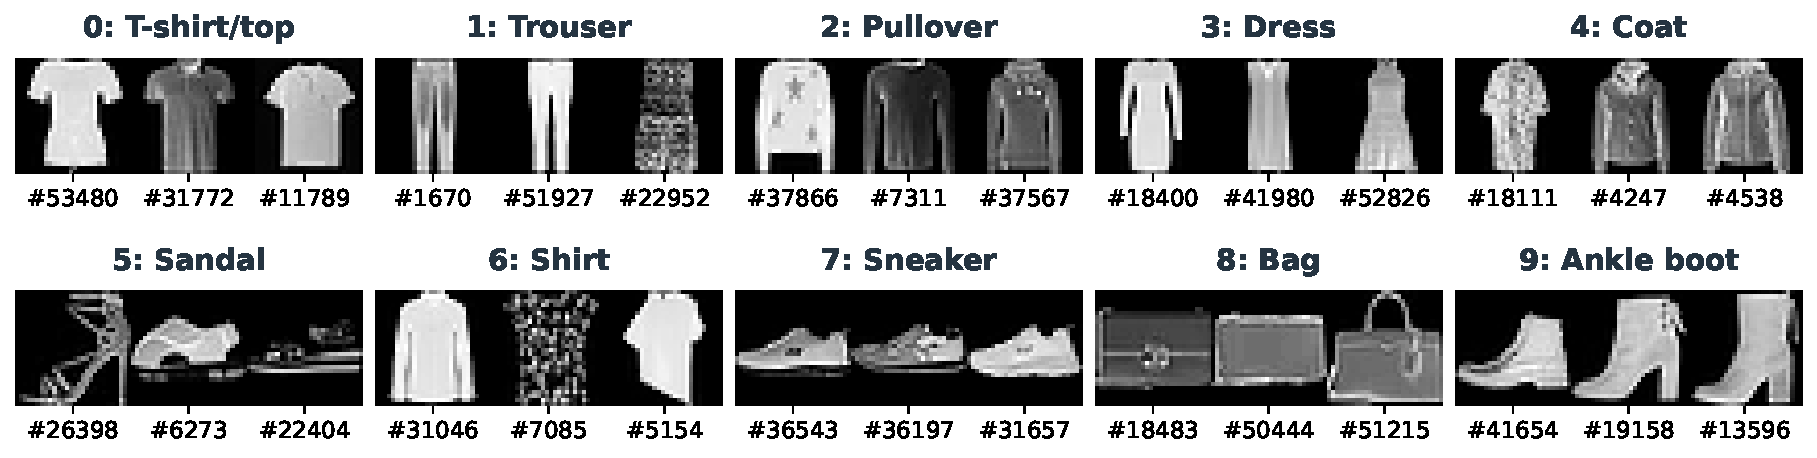
\includegraphics[width=.97\linewidth]{02_training_examples.pdf}
\caption{Three training examples per class. Numbers identify the original
training-source indices. All images use the same 0--255 display range.}
\label{fig:training_examples}
\end{figure}

\subsubsection{Pixel intensity and background}
The training subset contains 42,336,000 pixels. Their raw mean is 72.9833 and
their population standard deviation is 90.0557. Approximately 50.21\% of these
pixels are exactly zero, but none of the training images is entirely blank.
A large background region therefore does not indicate an empty sample.

\begin{figure}[H]\centering
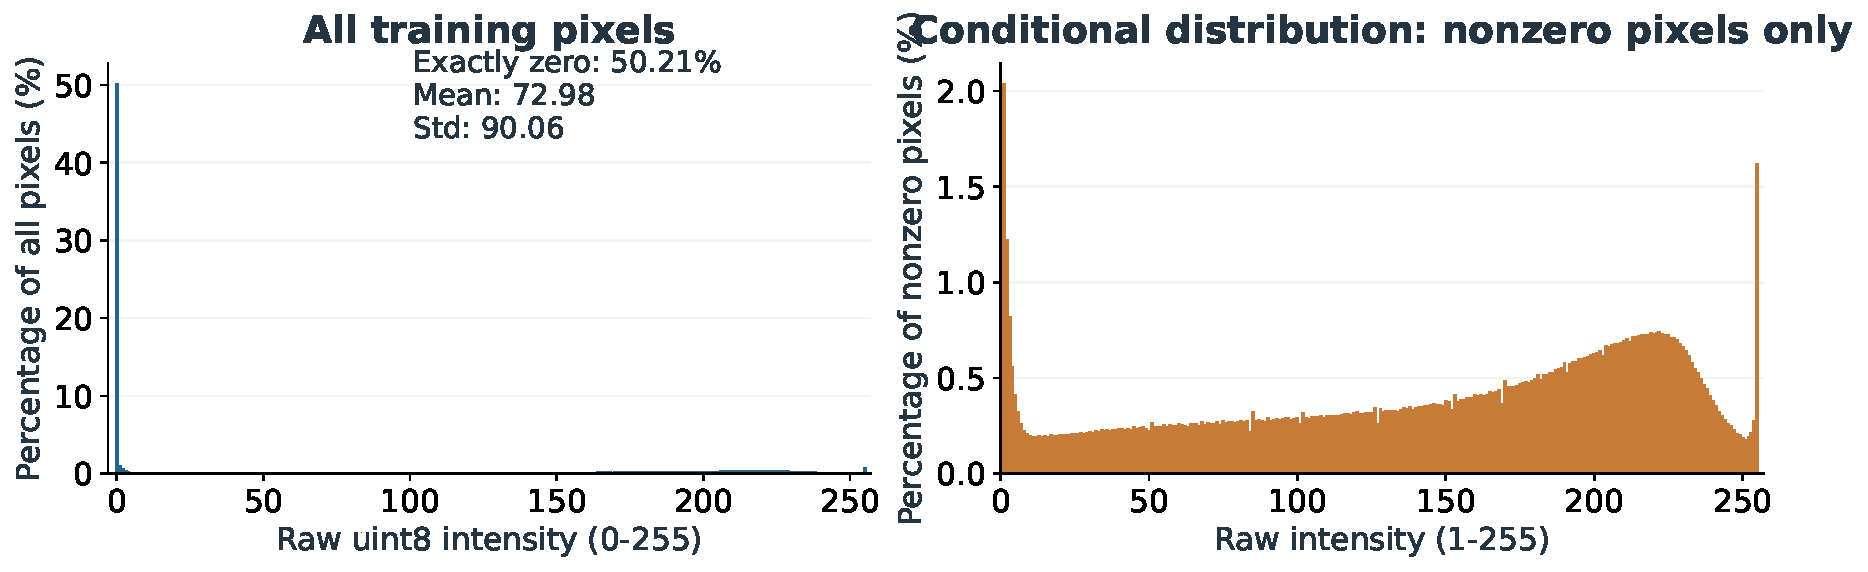
\includegraphics[width=.96\linewidth]{03_pixel_distribution.pdf}
\caption{Training-pixel intensity distributions. The left panel includes all
pixels; the right panel conditions on positive intensities. The panels use
different denominators.}\label{fig:pixels}
\end{figure}

The large zero-intensity mass is consistent with the dark background visible
in the samples. Positive pixels include both object interiors and faint edges.
Counting nonzero pixels is useful for describing coverage, but is not a semantic
segmentation of the clothing item.

\clearpage
\subsubsection{Brightness, coverage and spatial structure}
For each image, mean brightness is the average of its 784 raw intensities.
Nonzero coverage is the fraction of pixels with intensity greater than zero.
Table~\ref{tab:brightness} summarizes these quantities by class.

\begin{table}[H]\centering
\caption{Training statistics by class. Each row represents 5,400 images.
Brightness SD is the standard deviation of image means.}
\label{tab:brightness}
\begin{tabular}{lrrr}\toprule
Class & Mean brightness & Brightness SD & Nonzero coverage (\%)\\\midrule
\tabledata{generated/eda_rows.tex}
\bottomrule\end{tabular}
\end{table}

Sandal has the lowest mean brightness, 34.87, while Coat has the highest,
98.15. Pullover has the largest mean nonzero coverage, 64.84\%. These are
class averages, not decision rules: individual images vary and the class
distributions overlap.

\begin{figure}[H]\centering
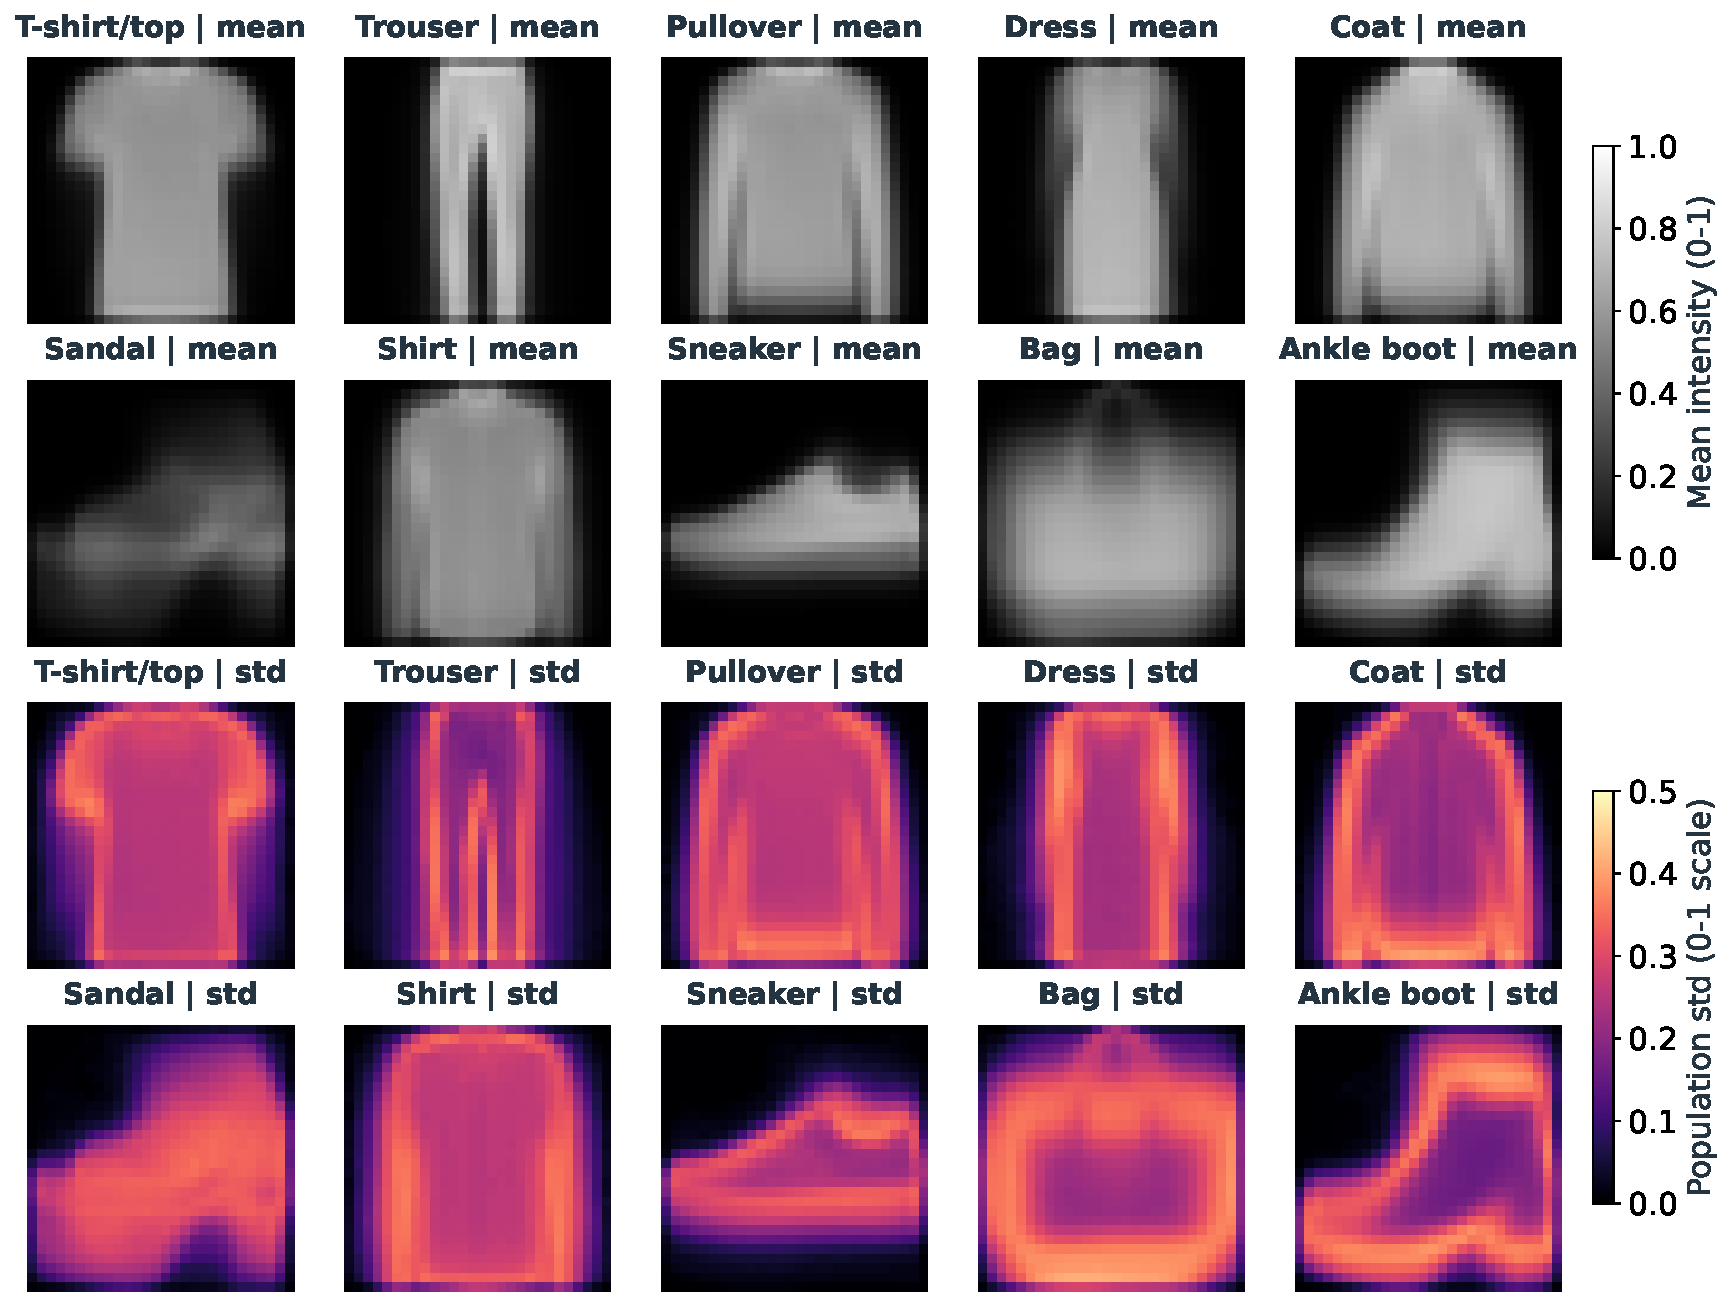
\includegraphics[width=.76\linewidth]{05_spatial_statistics.pdf}
\caption{Training class-average images and pixelwise standard deviations.
The average highlights recurring silhouettes; the standard deviation shows
where images within a class differ.}\label{fig:spatial}
\end{figure}

The class averages preserve broad silhouettes while removing much individual
detail. The recorded cosine similarity between the uncentered Coat and Shirt
averages is 0.9873, the highest pair in the audit. This suggests a useful question
for error analysis: do models confuse upper-body garments? It does not measure
the separability of individual images or prove a particular confusion rate.

\clearpage
\subsection{Preprocessing}
\label{sec:preprocessing}
\subsubsection{Scaling and training-only standardization}
Raw intensities are first converted to floating-point values and divided by 255.
The training mean $\mu$ and population standard deviation $\sigma$ are then
computed over all training pixels. For a raw pixel $X_{r,c}$, the normalized
value is
\[
Z_{r,c}=\frac{X_{r,c}/255-\mu}{\sigma},
\qquad \mu=0.286209,\quad \sigma=0.353160.
\]
The values shown are rounded; the code uses the full-precision cached constants.
Validation and test images reuse these constants without fitting their own
statistics. This prevents held-out images from influencing normalization.

The transformation preserves resolution and pixel ordering. Raw values 0 and
255 map to approximately $-0.810$ and $2.021$, without clipping.

\subsubsection{Input arrangements}
The same standardized image is rearranged to match each model:
Linear and MLP receive 784 pixels in row-major order; CNN receives a single
channel image grid; LSTM receives 28 top-to-bottom rows; and Transformer
receives 49 non-overlapping $4\times4$ patches in raster order.

\begin{figure}[H]\centering
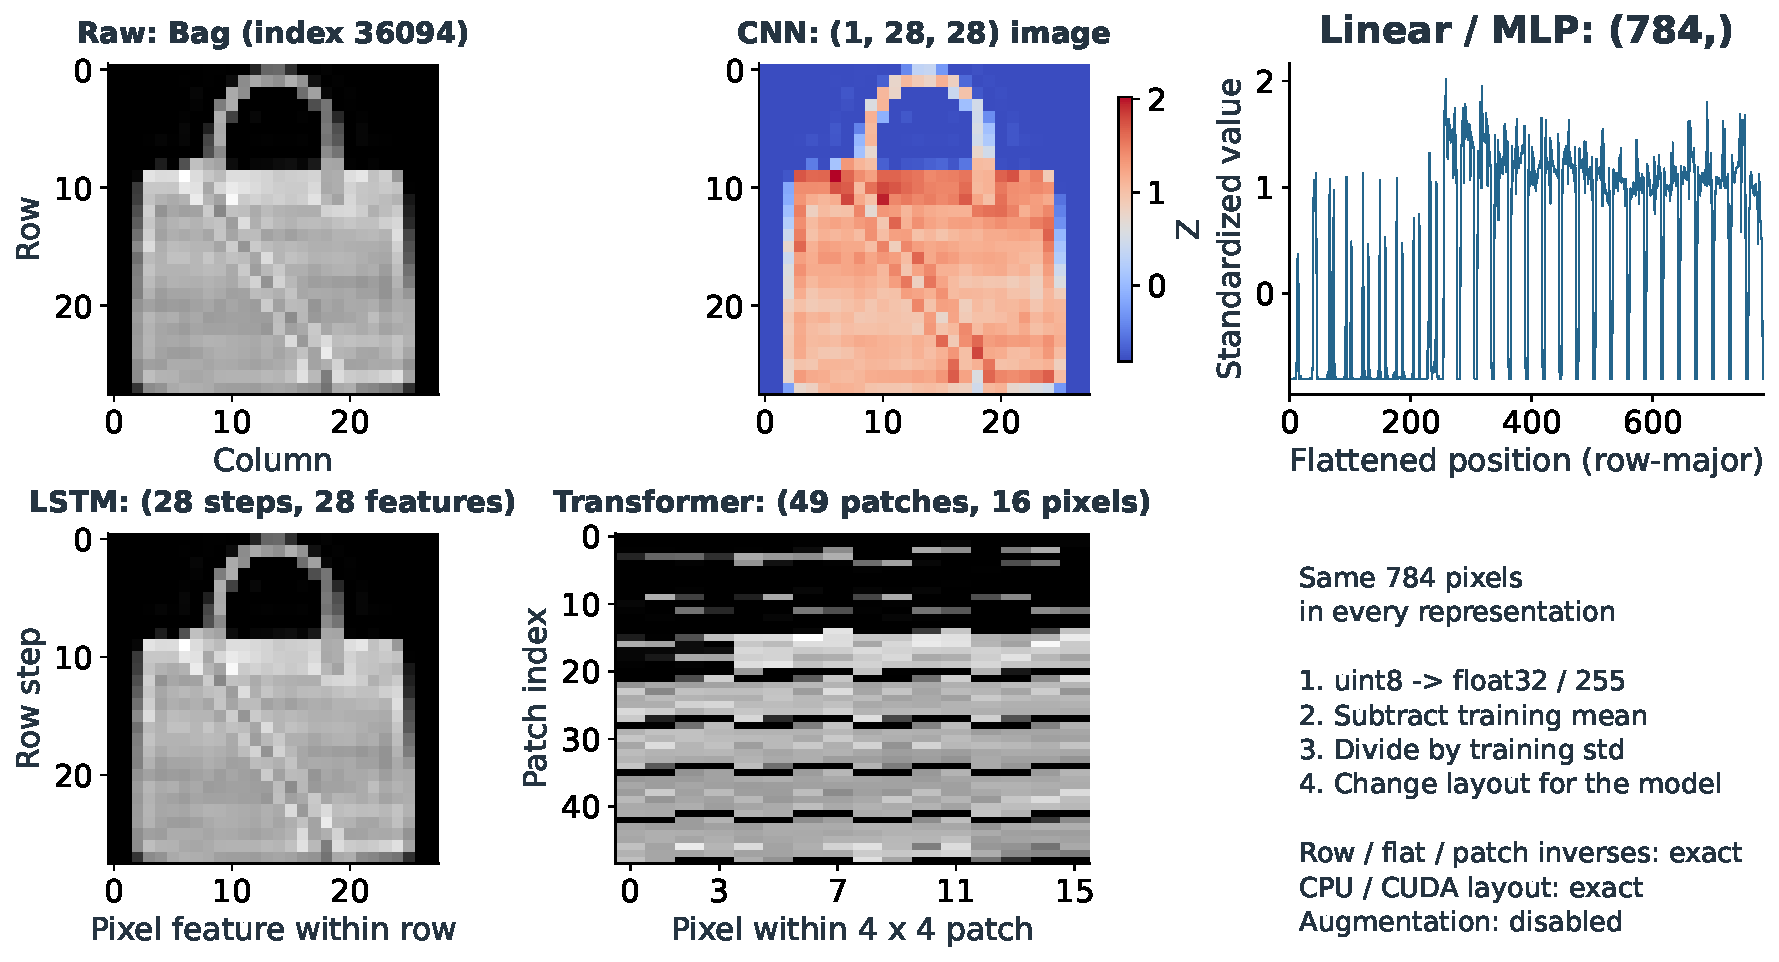
\includegraphics[width=.82\linewidth]{07_preprocessing_representations.pdf}
\caption{Equivalent input arrangements for the same image. Each arrangement
retains all 784 standardized pixel values. Learned embeddings belong to the
model, after preprocessing.}\label{fig:representations}
\end{figure}

For Transformer patch coordinates $a,b\in\{0,\ldots,6\}$ and local coordinates
$u,v\in\{0,\ldots,3\}$, the mapping is
\[
P_{7a+b,\,4u+v}=Z_{4a+u,\,4b+v}.
\]
Thus $49\times16=784$ values are retained without padding or interpolation.
For the LSTM, the sequence describes ordered positions in one static image;
it is not a time series of different images.

\subsubsection{Augmentation and verification}
No rotations, flips, resizing, denoising or other augmentation are applied.
The recorded preprocessing checks confirm that the standardized training data
has mean approximately zero and population standard deviation approximately
one, with deviations below $10^{-6}$. They also confirm pixel ordering, exact
patch reconstruction and CPU/CUDA agreement.

The following methodology compares ways of using this shared image information,
with particular interest in local structure and similar garment silhouettes.

\clearpage
% Fresh section. The retained report and earlier methodology are not edited.
% For integration, include this file after Section 2 and merge references.tex.
\section{Methodology}
\label{sec:fresh_methodology}
The experiment compares five ways of classifying a clothing image: Linear, MLP,
CNN, LSTM and Transformer. Each model receives the same image information, but
processes it differently. Linear and MLP use a pixel vector, CNN uses the image
grid, LSTM reads image rows, and Transformer works with small image patches.
This section describes the implemented models and the procedure used to train
and evaluate them.

\subsection{Shared data and workflow}
Fashion-MNIST contains ten classes of $28\times28$ grayscale images
\cite{fresh_fashion}. As described in Section~2, the official training set is
divided into 54,000 training images and 6,000 validation images using a
stratified split with seed~42. The official test set contains 10,000 images.
Training fits the model weights, validation chooses which saved weights to
keep, and testing measures the selected model.

All models use the preprocessing from Section~2. Pixel values are divided by
255 and standardized with the training mean and standard deviation,
approximately 0.286209 and 0.353160. The same constants are reused for validation
and testing. No images are resized, augmented or removed.

\begin{center}
\small
\begin{tabular}{c@{\quad$\longrightarrow$\quad}c@{\quad$\longrightarrow$\quad}c}
Standardized image & Model-specific input & Ten class scores\\[5pt]
\multicolumn{3}{c}{Training updates weights; validation selects weights; testing evaluates them.}
\end{tabular}
\end{center}

Table~\ref{tab:fresh_inputs} gives the input to each model. Here, $B$ is the
number of images in a batch. Each representation contains all 784 pixel values
per image. The labels are integer class indices from 0 to 9. Every model returns
a tensor of shape $(B,10)$ containing raw class scores, called logits.

\begin{table}[h]
\centering
\caption{Inputs and trainable parameter counts of the implemented models.}
\label{tab:fresh_inputs}
\begin{tabularx}{\linewidth}{l l X r}
\toprule
Model & Input shape & Arrangement & Parameters\\
\midrule
Linear & $(B,784)$ & One vector per image & 7,850\\
MLP & $(B,784)$ & One vector per image & 235,146\\
CNN & $(B,1,28,28)$ & One grayscale image grid & 421,642\\
LSTM & $(B,28,28)$ & 28 rows, each with 28 pixels & 82,186\\
Transformer & $(B,49,16)$ & 49 patches, each with 16 pixels & 71,946\\
\bottomrule
\end{tabularx}
\end{table}

\subsection{Pixel-based baselines}
\subsubsection{Linear classifier}
The Linear model assigns a weight to each pixel for each class. For a flattened
image $x\in\mathbb{R}^{784}$, its output is
\[
z=Wx+b,\qquad W\in\mathbb{R}^{10\times784},\quad b\in\mathbb{R}^{10}.
\]
The largest score determines the prediction. This model provides a small
baseline with no hidden layer. It can learn which pixel positions support a
class, but cannot learn nonlinear combinations of those pixels.

\subsubsection{Multilayer perceptron}
The MLP adds two hidden layers with 256 and 128 units. Each hidden layer is
followed by ReLU and dropout with probability 0.2. ReLU sets negative values to
zero, while dropout randomly suppresses some activations during training.
\[
784 \;\longrightarrow\; 256 \;\longrightarrow\; 128
\;\longrightarrow\; 10.
\]
The hidden layers allow the MLP to learn nonlinear relationships among pixels.
The image is still treated as a vector: nearby pixels do not receive a special
shared operation. Dropout is disabled during validation and testing.

\clearpage
\subsection{Models for spatial and sequential structure}
\subsubsection{Convolutional neural network}
The CNN keeps the two-dimensional image layout. Convolution applies the same
small filter at different image positions, allowing the network to learn local
patterns such as edges and contours \cite{fresh_cnn}. Our model has two
convolutional blocks, followed by a dense classifier.

Both convolutions use $3\times3$ kernels, stride~1 and padding~1, so they preserve
height and width. ReLU follows each convolution. A $2\times2$ max-pooling layer
then keeps the largest value in each window and halves both spatial dimensions.
The first block produces 32 feature maps and the second produces 64.

\begin{table}[h]
\centering
\caption{CNN operations and output sizes.}
\label{tab:fresh_cnn}
\begin{tabularx}{\linewidth}{X l}
\toprule
Operation & Output shape\\
\midrule
Input image & $(B,1,28,28)$\\
$3\times3$ convolution, 32 channels; ReLU & $(B,32,28,28)$\\
$2\times2$ max pooling & $(B,32,14,14)$\\
$3\times3$ convolution, 64 channels; ReLU & $(B,64,14,14)$\\
$2\times2$ max pooling & $(B,64,7,7)$\\
Flatten & $(B,3136)$\\
Dense layer, 128 units; ReLU; dropout 0.2 & $(B,128)$\\
Dense layer, 10 outputs & $(B,10)$\\
\bottomrule
\end{tabularx}
\end{table}

The final classifier combines the learned spatial features into ten scores.
Although convolution shares weights across positions, the dense layer from
3,136 features to 128 units accounts for most of this model's parameters.
The CNN therefore has the largest parameter count in this comparison.

\subsubsection{Row-sequence LSTM}
An LSTM maintains a hidden state and a memory state while reading a sequence
\cite{fresh_lstm}. Here, the sequence comes from a static image. The first step
receives the top row, the second receives the next row, and the last receives
the bottom row. Each step contains 28 pixel values.

For a standardized image $X$, row $t$ is
$r_t=X_{0,t,:}$. The batch shape $(B,28,28)$ means
\emph{batch, row steps, pixel features}. The two dimensions of size 28 have
different roles; the sequence is not a sequence of different images.

\begin{center}
\small
\begin{tabular}{c@{\ $\longrightarrow$\ }c@{\ $\longrightarrow$\ }c@{\ $\longrightarrow$\ }c}
Row 1 & Row 2 & $\cdots$ & Row 28\\
\multicolumn{4}{c}{One shared LSTM reads the rows in order.}\\[5pt]
\multicolumn{4}{c}{$h_{28}\in\mathbb{R}^{128}
\;\longrightarrow\; \text{dropout }0.2
\;\longrightarrow\; \text{dense layer}
\;\longrightarrow\; 10\text{ scores}$}
\end{tabular}
\end{center}

The implementation uses one forward LSTM layer with 128 hidden units. Its
hidden and memory states start at zero for each image. The gates control what
information is retained and updated as successive rows are read. After the
28th row, the final hidden state is passed through dropout and a linear
classifier. No state is carried from one image to another.

This design tests whether a compact summary built from ordered rows is useful
for classification. It introduces a top-to-bottom reading order, whereas the
CNN processes local neighborhoods throughout the image.

\clearpage
\subsection{Patch-based Transformer}
The Transformer uses attention to combine information from different parts of
an image \cite{fresh_attention}. The input follows the image-patch idea
\cite{fresh_vit}, using a small configuration suited to the $28\times28$ images.

\subsubsection{Patch tokens and position information}
Each image is divided into a $7\times7$ grid of non-overlapping $4\times4$
patches. Each patch is flattened into 16 values. Patches are ordered from left
to right across each row of the grid, then from top to bottom.
A learned linear layer maps each patch from 16 values to 64 features.
A learned positional vector is added so the model can distinguish patch
locations:
\[
e_j=Wp_j+b+q_j,\qquad j=1,\ldots,49,
\]
where $p_j\in\mathbb{R}^{16}$ is a patch,
$W\in\mathbb{R}^{64\times16}$ is the projection, and
$q_j\in\mathbb{R}^{64}$ is its position vector.
Dropout with probability 0.2 is applied after this addition.

\subsubsection{Attention blocks and classification}
Two encoder blocks process the 49 tokens. Each block uses four attention heads,
a feature width of 64, and a feedforward network with hidden width 128 and
GELU activation. Layer normalization is applied before each attention and
feedforward sublayer, with residual connections around both. Dropout is 0.2.

For one attention head, the operation is
\[
\operatorname{Attention}(Q,K,V)
=\operatorname{softmax}\left(\frac{QK^\top}{\sqrt{16}}\right)V.
\]
The queries $Q$, keys $K$ and values $V$ are learned projections of the tokens.
Each head has 16 features because the 64 features are divided among four heads.
Attention weights determine how much information one patch receives from the
others. All 49 patches are available to every patch; no causal mask is used.

\begin{table}[h]
\centering
\caption{Transformer representation through the network.}
\label{tab:fresh_transformer}
\begin{tabularx}{\linewidth}{X l}
\toprule
Stage & Shape\\
\midrule
Flattened image patches & $(B,49,16)$\\
Patch projection and learned positions & $(B,49,64)$\\
Two encoder blocks & $(B,49,64)$\\
Final layer normalization; mean over patches & $(B,64)$\\
Dropout 0.2; dense classifier & $(B,10)$\\
\bottomrule
\end{tabularx}
\end{table}

The final representation is the mean of the 49 normalized output tokens.
There is no extra classification token. The encoder internally uses
sequence-first tensors of shape $(49,B,64)$; this transpose changes the layout,
not the patch order. All weights are trained from scratch.

\subsection{Learning objective}
Every model learns to assign a high score to the correct class. For image $i$,
softmax converts the logits $z_{i,k}$ into class probabilities:
\[
p_{i,k}=\frac{\exp(z_{i,k})}{\sum_{j=0}^{9}\exp(z_{i,j})},
\qquad
\mathcal{L}=-\frac{1}{B}\sum_{i=1}^{B}\log p_{i,y_i}.
\]
Here, $y_i$ is the correct class and $\mathcal{L}$ is the average cross-entropy
loss. The implementation passes logits directly to
\texttt{CrossEntropyLoss}, which performs the required calculation.
Prediction uses $\hat y_i=\arg\max_k z_{i,k}$. Class weights are not used because
the training split contains the same number of examples from each class.

\clearpage
\subsection{Training procedure}
All five models use Adam \cite{fresh_adam} with learning rate 0.001, batch size
128 and a budget of ten epochs. These settings give each model the same number
of passes over the training data. Table~\ref{tab:fresh_training} records the
shared choices.

\begin{table}[h]
\centering
\caption{Training and checkpoint selection settings.}
\label{tab:fresh_training}
\begin{tabularx}{\linewidth}{l X}
\toprule
Setting & Value\\
\midrule
Random seed & 42 for Python, NumPy, PyTorch and the training shuffle\\
Optimizer & Adam, learning rate 0.001\\
Batch size & 128; the smaller last batch is kept\\
Training duration & 10 complete epochs\\
Loss & Unweighted cross-entropy\\
Regularization & Dropout 0.2 in MLP, CNN, LSTM and Transformer\\
Checkpoint selection & Lowest validation loss; an exact tie keeps earlier weights\\
Data loading & Training shuffled; validation and test ordered; zero workers\\
Other settings & No augmentation, weight decay, gradient clipping or scheduler\\
\bottomrule
\end{tabularx}
\end{table}

Each model is initialized separately after resetting the seed. A training epoch
visits all 54,000 training images. For each batch, the program clears the
previous gradients, calculates the logits and loss, backpropagates, and updates
the weights with Adam.

At the end of the epoch, the model is evaluated on all 6,000 validation images.
Evaluation mode disables dropout, and gradient recording is turned off.
The program saves the weights whenever validation loss improves. Training
continues through epoch ten, even if the best checkpoint was found earlier.
The saved checkpoint with the lowest validation loss is then reloaded for
testing.

Epoch loss is weighted by the number of images in each batch, so a smaller final
batch does not receive the same weight as a full batch. Accuracy and macro-F1
are calculated from predictions across the complete split. Training metrics
are collected while the weights change; validation metrics use the fixed
weights at the end of an epoch.

\subsection{Evaluation measures}
The selected checkpoint is evaluated on all 10,000 official test images.
Accuracy measures the fraction classified correctly:
\[
\operatorname{Accuracy}=\frac{1}{N}\sum_{i=1}^{N}
\mathbf{1}(\hat y_i=y_i).
\]
Here, $N$ is the number of evaluated images and $\mathbf{1}$ is one when the
prediction is correct, otherwise zero.

Macro-F1 gives equal weight to every class. For class $k$, true positives
$TP_k$ are correct predictions of that class, false positives $FP_k$ are other
classes predicted as $k$, and false negatives $FN_k$ are examples of $k$
predicted as another class:
\[
F1_k=\frac{2TP_k}{2TP_k+FP_k+FN_k},
\qquad
\operatorname{MacroF1}=\frac{1}{10}\sum_{k=0}^{9}F1_k.
\]
Undefined class scores are assigned zero. Both accuracy and macro-F1 are
reported because overall accuracy alone does not show how performance varies
among categories.

The evaluation also saves cross-entropy loss, per-class precision and recall,
and a confusion matrix. Matrix rows represent true labels and columns represent
predicted labels. Correct and incorrect example images help explain recurring
mistakes. These outputs support the results and error analysis; they do not
select the training checkpoint.

\clearpage
\subsection{Runtime, reproducibility and comparison scope}
\subsubsection{Runtime measurements}
Training time covers the ten-epoch training and validation loop, including
saving improved checkpoints. It excludes data preparation before the loop and
the final checkpoint reload and validation after it.

Forward-pass timing uses a fixed batch of 128 images already on the device.
After ten warm-up calls, the program times 100 forward calls and averages their
duration. Dividing the batch time by 128 gives time per image at that batch
size. Device synchronization is performed around the timed region. This
measurement excludes data loading and host-to-device transfers and describes
batched throughput, not the latency of a single-image request.

A separate timer measures the complete test pass, including loading, transfers,
model execution, loss and prediction collection. It excludes later metric
summaries and plots. The two measurements are reported separately because they
cover different work.

\subsubsection{Reproducibility}
The implementation separates data preparation in \texttt{a1/data.py}, model
definitions in \texttt{a1/models.py}, training in \texttt{a1/train.py}, and testing
in \texttt{a1/evaluate.py}. Configuration files specify the shared training
settings. The split cache records the training and validation indices and the
normalization constants.

Each run saves the selected checkpoint, epoch history and a summary of its
configuration and environment. Evaluation checks the recorded data and split
hashes and normalization values before using the checkpoint. It also saves
per-image predictions so that the reported scores can be checked again.

The following commands illustrate the CNN workflow from the \texttt{A1} folder
with the project dependencies installed. The other models use the same entry
points and their corresponding configuration files.
\begin{quote}\small\ttfamily
python -m a1.train --model cnn --config configs/cnn.json\\
python -m a1.evaluate --checkpoint runs/m2/cnn/best.pt --device cuda
\end{quote}

\subsubsection{What the comparison can establish}
The split, preprocessing, seed, optimizer, learning rate, batch size and epoch
budget are shared. The architecture, input arrangement and parameter count
change. The experiment therefore compares these five implemented configurations.
It does not hold model capacity or computation constant.

All computational-cost measurements in Section~\ref{sec:results} use CUDA on
an NVIDIA GeForce GTX 1660 SUPER. Linear and MLP were repeated on CUDA with
the same seed, split and training protocol, in separate run directories.
The classification scores and error analysis retain the original selected
checkpoints; the baseline cost rows describe these separate CUDA repetitions.
Finally, each model has one recorded
training seed. Differences in the resulting scores describe these runs; repeated
seeds would be needed to measure how much the results vary.


\clearpage
\section{Experimental Results}
\label{sec:results}
\subsection{Overall classification performance}
Table~\ref{tab:results} compares the validation-selected checkpoints.
Validation accuracy describes the 6,000-image selection partition; test
accuracy describes the separate 10,000-image official test partition.
All test metrics refer to the same ordered images.

\begin{table}[H]\centering
\caption{Results of the five saved runs. Accuracy is a percentage;
macro-F1 is on the 0--1 scale. Epoch is selected by validation loss.}
\label{tab:results}
\small
\begin{tabular}{lrrrrrr}\toprule
Model & Epoch & Val.\ acc. & Test acc. & Test F1 & Test loss & Errors\\\midrule
\tabledata{generated/results_rows.tex}
\bottomrule\end{tabular}
\end{table}

The CNN has the highest test accuracy and macro-F1, and the lowest test loss.
Its 91.94\% accuracy is 3.44 percentage points above the MLP and 7.68 points above
the Linear model. Relative to the MLP, it reduces the number of mistakes from
1,150 to 806, a reduction of 344 images or 29.9\% of the MLP's errors.

The MLP improves over Linear by 4.24 percentage points. Adding nonlinear hidden
layers is therefore useful in this experiment, even though both models use the
same flattened input. The CNN improves further while retaining spatial
neighborhoods, but its larger capacity also changes the comparison.

\begin{figure}[H]\centering
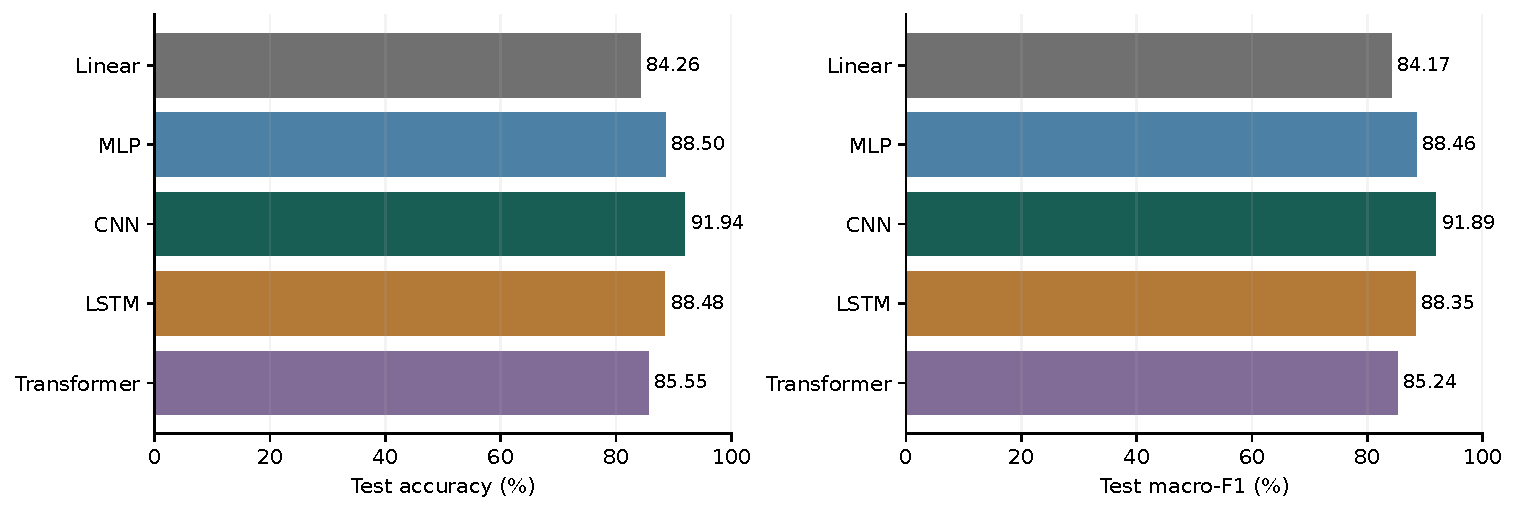
\includegraphics[width=\linewidth]{test_comparison.pdf}
\caption{Official-test accuracy and macro-F1, both displayed as percentages.
Axes start at zero. These are single-run scores, without repeated-seed error bars.}
\label{fig:comparison}
\end{figure}

MLP and LSTM are almost tied: their test accuracies differ by 0.02 percentage
points, or two images. This is too small to support a stable ranking without
repeated runs. Their macro-F1 values are also close, although their class-level
mistakes differ.

The Transformer obtains 85.55\% test accuracy, 1.29 percentage points above
Linear and below the other nonlinear models. This result describes the small,
two-block patch model trained for ten epochs. It does not establish that
attention-based image models are generally weaker than CNNs or MLPs.

Because the test set has equal class support, weighted F1 and macro-F1 are
identical here. Accuracy and macro-F1 remain different measures: F1 also
depends on how false positives are distributed across classes.

\clearpage
\subsection{Learning behavior and checkpoint selection}
Figure~\ref{fig:curves} shows the recorded training and validation losses for
all ten epochs. The same vertical scale is used for every model.

\begin{figure}[H]\centering
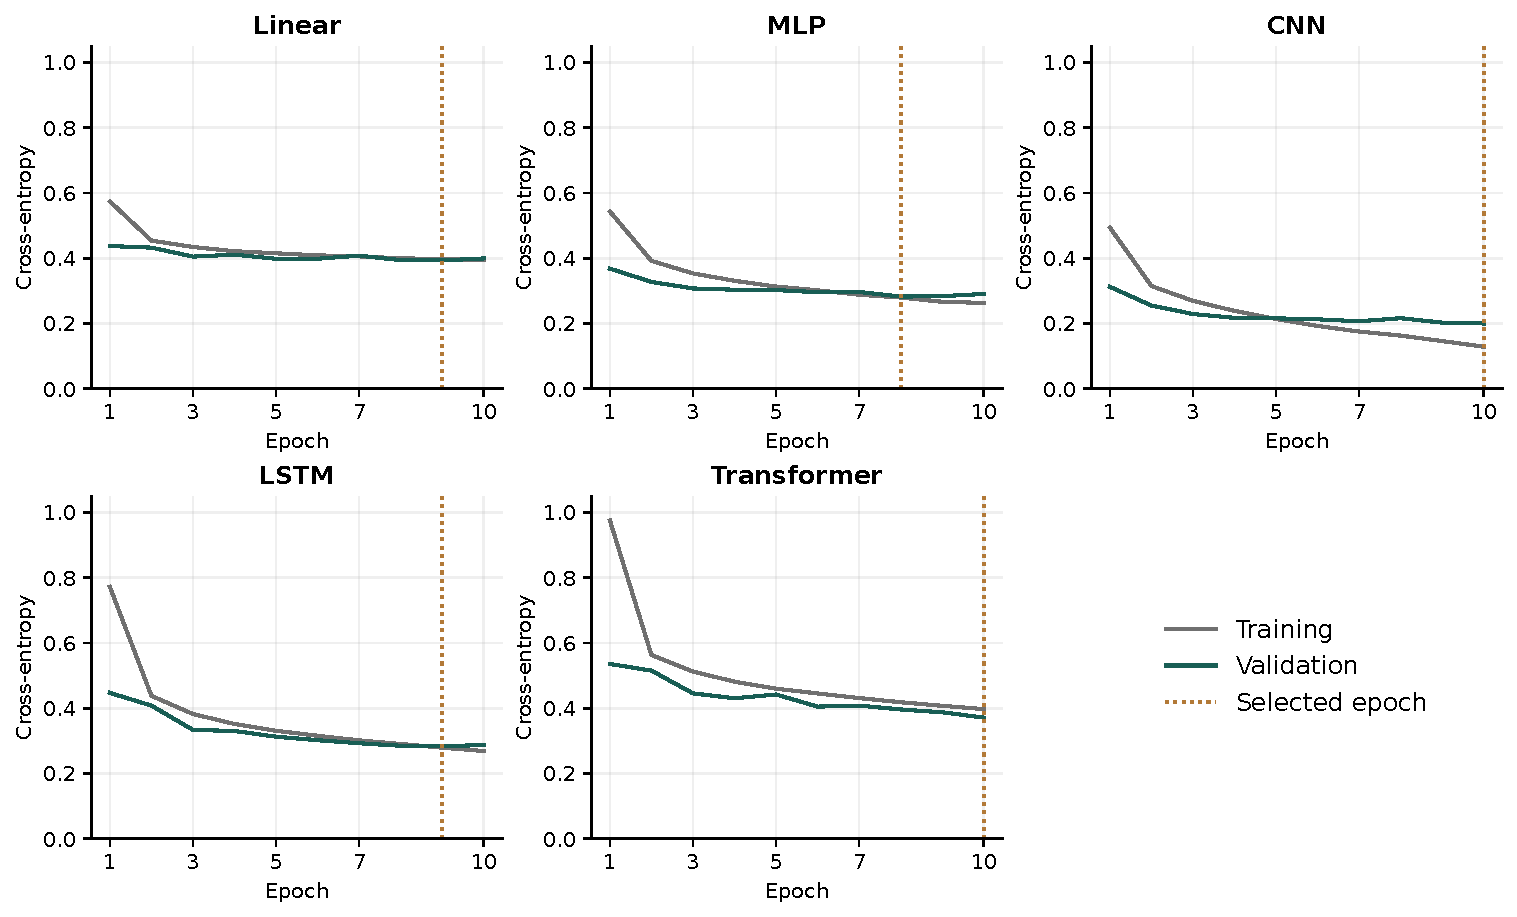
\includegraphics[width=\linewidth]{learning_curves.pdf}
\caption{Cross-entropy over ten epochs. Dotted lines mark the checkpoint with
the lowest validation loss. Training loss is collected with dropout active
and changing weights; validation loss uses evaluation mode after each epoch.}
\label{fig:curves}
\end{figure}

\begin{table}[H]\centering
\caption{First and final validation losses, with final-epoch accuracies.
These final-epoch values need not belong to the selected checkpoint.}
\label{tab:history}
\small
\begin{tabular}{lrrrr}\toprule
Model & Val.\ loss, epoch 1 & Val.\ loss, epoch 10 & Train acc.\ (\%) & Val.\ acc.\ (\%)\\\midrule
\tabledata{generated/history_rows.tex}
\bottomrule\end{tabular}
\end{table}

All five models reduce validation loss between the first and last epochs.
Linear changes relatively little after its early improvement and selects
epoch 9. MLP selects epoch 8: its training loss continues to decrease, but its
validation loss rises from 0.2825 at epoch 8 to 0.2906 at epoch 10.
LSTM selects epoch 9 and also shows a small validation-loss increase at epoch 10.
These patterns support keeping the best checkpoint rather than automatically
using the last one.

CNN and Transformer select epoch 10. The Transformer is still improving at
the budget boundary, so the available run cannot show whether a longer schedule
would close the gap. For CNN, the final training accuracy is 95.19\% and validation
accuracy is 93.28\%, indicating a gap on these recorded metrics.

Validation loss can be lower than training loss, especially early in a run.
Dropout is disabled during validation, and validation uses weights after the
epoch rather than the changing weights seen throughout training.
The two curves should therefore not be treated as identical measurement conditions.

\clearpage
\subsection{Model size and computational cost}
\begin{table}[H]\centering
\caption{Parameter count and recorded CUDA runtime on GTX 1660 SUPER.
Linear and MLP costs use separate CUDA repetitions of the baseline protocol.
Forward time covers one
128-image device-resident batch on GTX 1660 SUPER. Test-pass time covers all
10,000 images, including loading, transfers, loss and prediction collection.}
\label{tab:runtime}
\small
\begin{tabular}{lrrlrr}\toprule
Model & Parameters & Train (s) & Train device & Forward (ms) & Test pass (s)\\\midrule
\tabledata{generated/runtime_rows.tex}
\bottomrule\end{tabular}
\end{table}

Linear is the smallest model, with 7,850 parameters, and has the shortest
recorded forward time. MLP uses 235,146 parameters.
CNN has 421,642 parameters and takes 1.074 milliseconds per batch.
The CNN's accuracy gain therefore comes with greater model size and forward
cost compared with these baselines.

LSTM and Transformer are smaller than the MLP, with 82,186 and 71,946 parameters,
but their recorded forward times are longer. Parameter count alone does not
describe execution cost. The LSTM processes 28 recurrent steps, and the
Transformer applies attention and feedforward operations to 49 tokens.
Kernel implementation and the chosen batch size also affect runtime.

\subsubsection{Interpreting training time}
All five training durations in Table~\ref{tab:runtime} were measured on CUDA
using the GTX 1660 SUPER. Linear and MLP were retrained with the same seed 42,
54,000/6,000 split, normalization, batch size 128, Adam learning rate 0.001,
and ten-epoch budget. Their new checkpoints and evaluations are saved under
\texttt{runs/cuda\_baselines}. The original baseline runs are retained for the
classification tables and error analysis. These two repetitions measure
computational cost and do not replace the original accuracy results.

For the other three CUDA runs, recorded training durations are 105.03 seconds for
CNN, 122.12 seconds for LSTM and 139.45 seconds for Transformer. These are the
observed durations for the shared ten-epoch budget, not estimates of average
runtime across repeated trials. The runs were recorded in separate sessions;
common hardware does not remove variation from system load or GPU clocks.

\subsubsection{Interpreting inference time}
All five saved inference measurements use the GTX 1660 SUPER, batch size 128,
ten warm-up calls and 100 timed forward calls. The data is already on the GPU.
The reported batch time excludes loading and host-to-device transfers.
For CNN, 1.074 milliseconds per batch corresponds to approximately
0.00839 milliseconds per image \emph{within that batch}. It is not the latency
of a single-image request.

The complete test pass includes the additional work shared by the evaluation
pipeline. Because the forward and test-pass timers cover different operations,
they should not be subtracted to estimate an exact loading overhead.

The saved summaries do not contain model-specific peak GPU memory or energy
measurements. Parameter counts are reported directly, without treating them
as a substitute for those missing resource measurements.

\clearpage
\section{Error Analysis}
\label{sec:errors}
\subsection{Performance by class}
The overall scores conceal substantial variation among categories.
Figure~\ref{fig:class_f1} compares the per-class F1 values of all five models.
The full numerical table is included in Appendix~A.

\begin{figure}[H]\centering
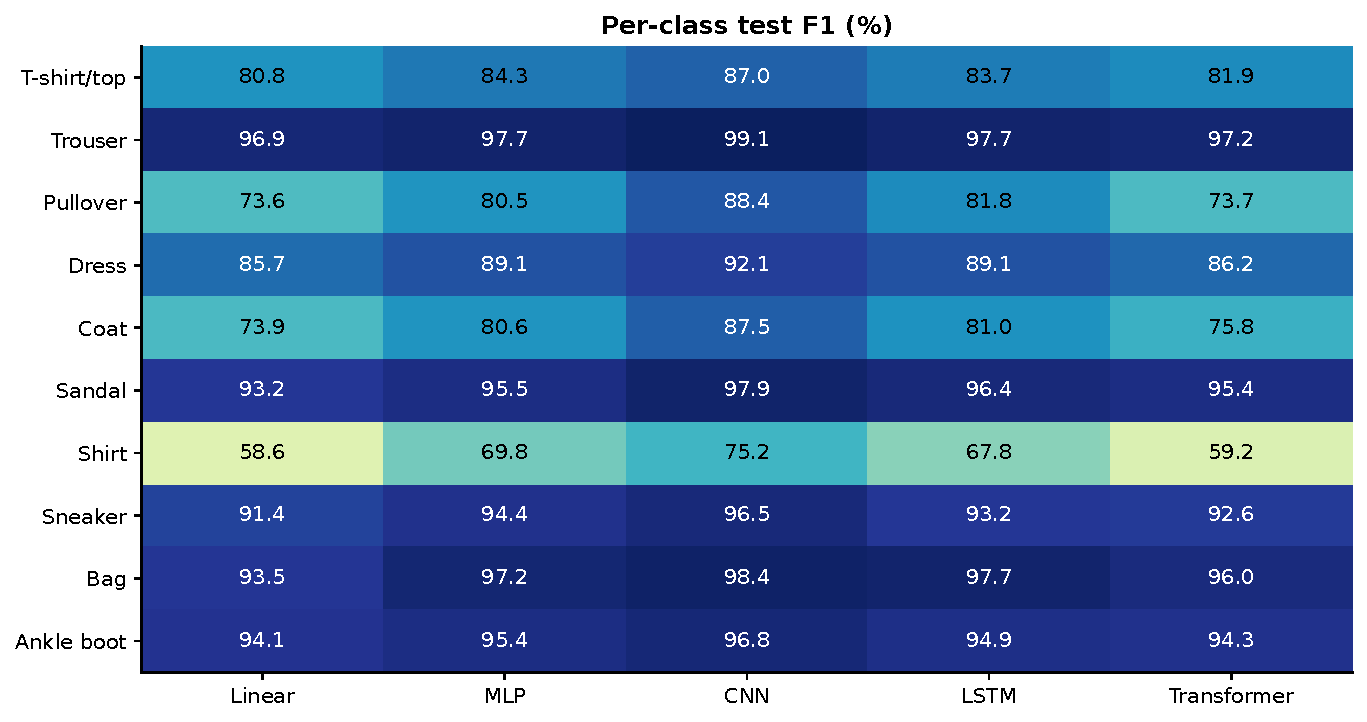
\includegraphics[width=.96\linewidth]{class_f1.pdf}
\caption{Per-class F1 on the official test set, shown as percentages.
Every class has 1,000 test images.}\label{fig:class_f1}
\end{figure}

Shirt has the lowest F1 for every model. Its score rises from 58.59\% for Linear
to 69.76\% for MLP and 75.18\% for CNN. Transformer reaches 59.20\%, which is
close to Linear on this class despite its higher overall score.

CNN has the highest F1 for each of the ten classes in the recorded runs.
Its improvement over MLP is particularly clear for Pullover
(80.54\% to 88.43\%) and Coat (80.65\% to 87.45\%).
For Trouser, both models already perform well, so the gain is smaller.

The LSTM's aggregate result is close to the MLP's, but it has higher F1 on
Pullover, Coat, Sandal and Bag, and lower F1 on Shirt and Sneaker.
For example, LSTM obtains 96.40\% F1 on Sandal versus 95.50\% for MLP,
but 67.84\% on Shirt versus 69.76\%.
The near tie in accuracy therefore does not mean the two models make the same
decisions.

These results broadly agree with the visual observations in Section~2:
upper-body categories are difficult to separate, while trousers and several
accessory or footwear categories are easier. However, class-average similarity
is only a descriptive summary. Models predict individual images, whose shapes
and textures can differ substantially from the average.

\clearpage
\subsection{Confusion patterns in the CNN}
Figure~\ref{fig:cnn_confusion} shows the CNN's confusion matrix. Rows are true
labels and columns are predicted labels. Each row contains 1,000 images.

\begin{figure}[H]\centering
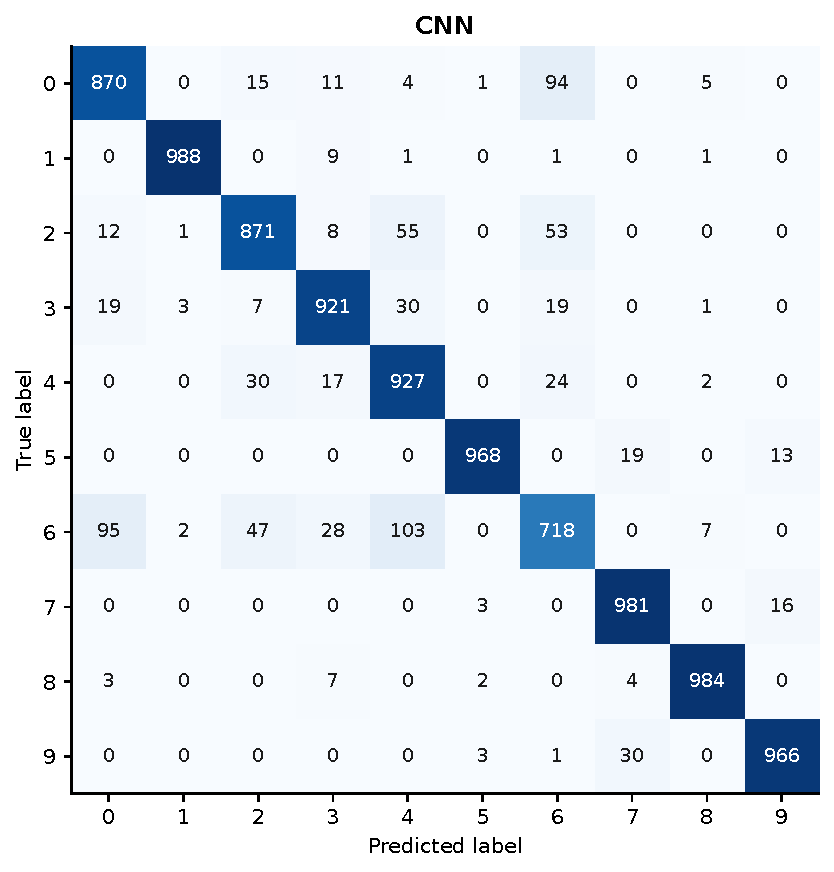
\includegraphics[width=.63\linewidth]{cnn_confusion.pdf}
\caption{CNN test confusion counts. Label IDs follow Table~\ref{tab:labels}.
The diagonal contains correct predictions.}\label{fig:cnn_confusion}
\end{figure}

\begin{table}[H]\centering
\caption{Six CNN class pairs with the largest combined two-way confusion.
The two directions are counted separately.}\label{tab:confusion_pairs}
\begin{tabular}{llrr}\toprule
Class A & Class B & A predicted as B & B predicted as A\\\midrule
\tabledata{generated/confusion_rows.tex}
\bottomrule\end{tabular}
\end{table}

Of the CNN's 806 mistakes, \UpperErrors{} occur between the four labels
T-shirt/top, Pullover, Coat and Shirt. These account for
\UpperErrorPercent\% of all errors. Shirt alone has 282 incorrect predictions:
103 become Coat, 95 become T-shirt/top and 47 become Pullover.

The confusions are not always symmetric. There are 103 Shirt-to-Coat errors
but only 24 Coat-to-Shirt errors. CNN recalls 92.7\% of Coat images, yet its
Coat precision is lower, at 82.77\%, because other garments are also predicted
as Coat. This distinction explains why recall alone would give an incomplete
view of the class.

\clearpage
\subsection{Individual predictions and shared errors}
Figure~\ref{fig:examples} displays four correct and four incorrect CNN
predictions. A seeded generator selects from the correct set and then the
incorrect set. The deliberately balanced display illustrates behavior; it
does not represent the model's actual error frequency.

\begin{figure}[H]\centering
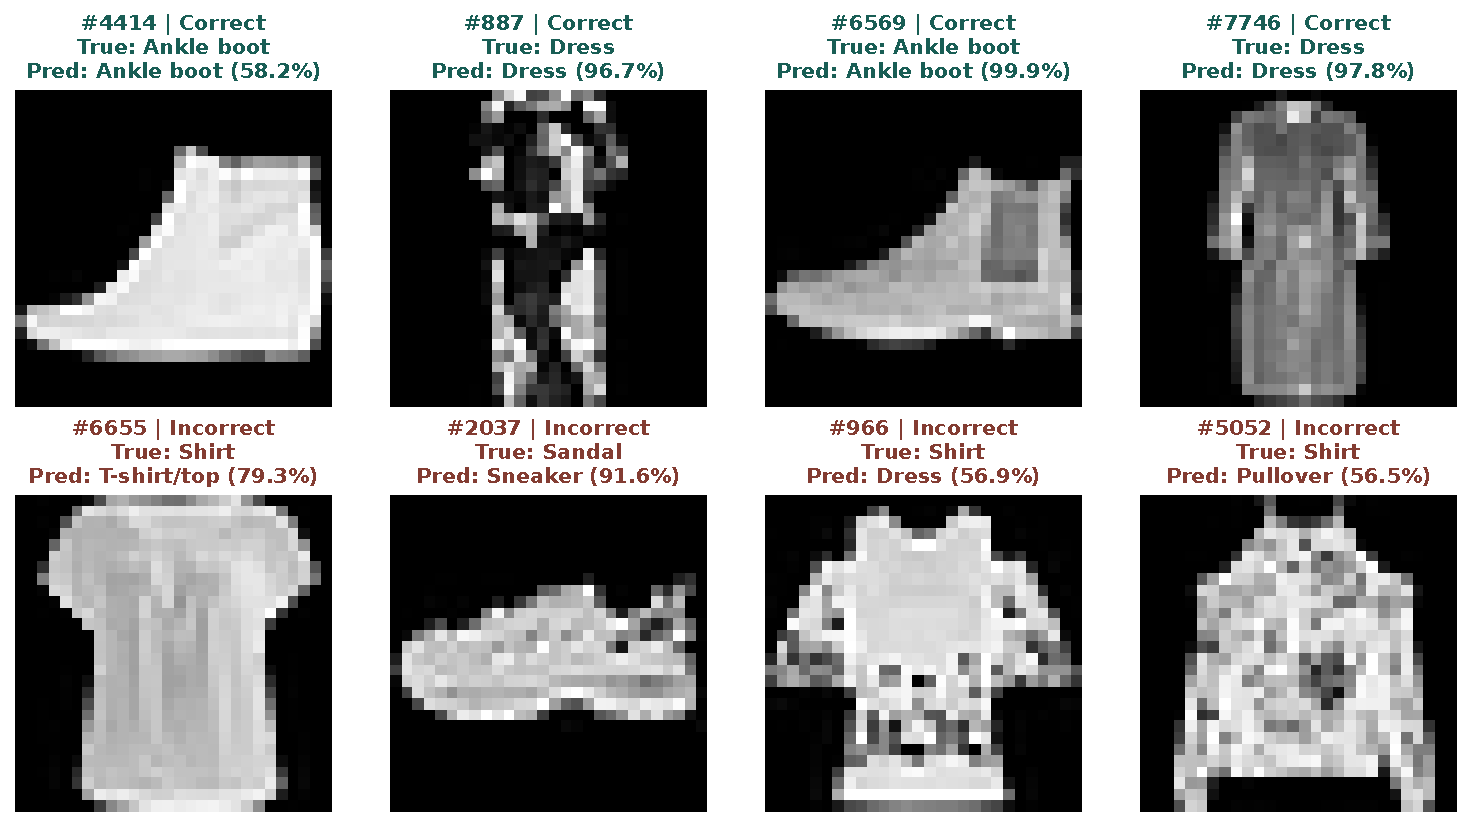
\includegraphics[width=.94\linewidth]{cnn_examples.pdf}
\caption{CNN examples from the official test set, sampled with seed 42.
Indices are zero-based test indices. The percentage is the maximum softmax
score, not a calibrated probability of correctness.}\label{fig:examples}
\end{figure}

Image \#6655 has a short-sleeved outline and is labeled Shirt, but is predicted
as T-shirt/top. Image \#5052 is also Shirt and is predicted as Pullover.
These examples illustrate the upper-body confusion counted in the matrix.
The images alone cannot reveal the model's internal reason for each decision.

The Sandal image \#2037 is predicted as Sneaker with a score of 91.6\%.
In contrast, the correctly classified Ankle boot \#4414 has a score of 58.2\%.
High confidence can accompany an error, and moderate confidence can accompany
a correct prediction. The study does not include a calibration experiment.

\begin{table}[H]\centering
\caption{Paired correctness on the same 10,000 test images.
``Only'' means the named model is correct and the other is wrong.}
\label{tab:paired}
\begin{tabular}{lrrr}\toprule
Compared with CNN & CNN only correct & Other only correct & Both wrong\\\midrule
\tabledata{generated/paired_rows.tex}
\bottomrule\end{tabular}
\end{table}

CNN corrects 566 images that MLP gets wrong, but MLP correctly handles 222 images
that CNN misses. The net difference is the 344-image advantage in Table~\ref{tab:results}.
MLP and LSTM also differ on individual cases: MLP alone is correct on
\MlpOnly{} images and LSTM alone on \LstmOnly{}, producing their two-image net gap.
All five models are wrong on \SharedErrors{} shared images.

These complementary decisions motivate future ensemble experiments, but no
ensemble has been trained or evaluated here. The paired counts describe
agreement and disagreement; they are not an achieved ensemble score.

\clearpage
\section{Discussion and Limitations}
\subsection{What the comparison shows}
The strongest result comes from the CNN. Its local filters and pooling provide
a natural way to process the spatial structure of clothing images.
The class-level results show gains across all categories, including the
similar upper-body garments that trouble the baselines. This is consistent
with the usefulness of local spatial features in this task.

That explanation remains an interpretation. The CNN also has the largest
parameter count, and no ablation isolates the contribution of convolution,
pooling, width or regularization. The experiment demonstrates a better result
for this configuration, rather than proving a single cause for the improvement.

The MLP is a useful practical baseline. It improves substantially over Linear
and nearly matches the LSTM while requiring less recorded forward time.
The LSTM achieves similar overall accuracy with fewer parameters, but reading
the image sequentially does not provide an accuracy advantage in this run.
Its final hidden state must summarize the rows before classification.

The Transformer has the fewest parameters among the four nonlinear models,
but it has the longest recorded forward time and a lower test score than MLP,
CNN or LSTM. Attention is not automatically an improvement under a small,
fixed training configuration. Since its validation loss is still decreasing
at epoch 10, longer training is a plausible follow-up, not an established remedy.

\subsection{Limits of the evidence}
\begin{enumerate}
\item \textbf{One seed per model.} The report does not estimate variation from
initialization or data ordering. Small score differences, especially between
MLP and LSTM, should not be treated as stable.
\item \textbf{Unequal capacity and computation.} The models share an epoch budget
but have different parameter counts, operations and training durations.
The study is not a capacity-matched or compute-matched ablation.
\item \textbf{Restricted optimization.} There is no systematic learning-rate,
width, dropout or schedule search. A shared setting may suit some models better
than others, and ten epochs need not be sufficient for every configuration.
\item \textbf{Hardware and timing scope.} All cost measurements use CUDA on
the GTX 1660 SUPER. Baseline costs come from separate repetitions; classification
scores retain the original checkpoints. Inference uses only one batch size and a short benchmark,
without repeated-session timing variation. Peak model memory is not recorded.
\item \textbf{Limited image domain.} Fashion-MNIST contains small grayscale
images. The experiment does not measure robustness to color, backgrounds,
occlusion, new product styles or distribution shift.
\item \textbf{Post-evaluation analysis.} Confusions and example images explain
the existing results. They do not justify tuning against the test set and
reporting the same set as an untouched final evaluation.
\end{enumerate}

\subsection{Next experiments}
The first priority is to repeat each configuration across several seeds and
report the mean and variation of accuracy and macro-F1. Training-speed
comparisons should repeat all five models in controlled sessions on the same
hardware and timing scope to quantify runtime variation.

Next, use validation data to compare longer schedules and modest learning-rate
changes, especially for Transformer. Separate ablations can examine CNN width,
LSTM readout and patch size while controlling one factor at a time.
Augmentation and calibration are further candidates. Any new settings should
be selected through validation before a clearly documented final evaluation.

\clearpage
\section{Conclusion}
This project compares five neural network configurations through a common
Fashion-MNIST pipeline. The data is split into fixed training, validation and
test partitions, normalized using training statistics, and presented as
vectors, image grids, row sequences or patch sequences. All models use the
same ten-epoch training budget and validation-loss checkpoint rule.

The CNN gives the strongest recorded result: 91.94\% test accuracy and
0.9189 macro-F1. It makes 806 errors on 10,000 images, 344 fewer than the MLP.
Its improvement appears across all ten class F1 scores, although Shirt remains
difficult, with 71.8\% recall. Most remaining CNN errors occur among
T-shirt/top, Pullover, Coat and Shirt.

MLP and LSTM obtain nearly equal accuracy at 88.50\% and 88.48\%. Their
two-image difference is too small to support a general ranking, and their
individual predictions differ substantially. Transformer reaches 85.55\%,
above the Linear baseline at 84.26\%, but below the other nonlinear models
under this configuration and training budget.

For this assignment, CNN is the preferred configuration when test accuracy
is the main criterion. MLP is a useful alternative when the recorded forward
cost matters: it trades some accuracy for a substantially shorter batch
forward time. LSTM is smaller than MLP in parameter count, but that smaller
count does not translate into faster measured inference.

The broader lesson is that a more elaborate architecture does not guarantee
a better result under a fixed experimental budget. Input structure, capacity,
optimization and runtime must be considered together. Repeated seeds and
controlled follow-up experiments are needed before these single-run findings
can be extended into stronger claims.

\vspace{8pt}
\begin{table}[H]\centering
\caption{Main findings and the evidence that supports them.}
\begin{tabularx}{\linewidth}{lX}\toprule
Finding & Evidence in this study\\\midrule
CNN leads in predictive quality &
91.94\% accuracy, 0.9189 macro-F1 and the highest F1 in each class.\\
MLP and LSTM are nearly tied &
88.50\% versus 88.48\% accuracy; no repeated-seed estimate.\\
Upper-body garments remain difficult &
\UpperErrors{} of the CNN's 806 errors occur within four upper-body labels.\\
Parameter count does not rank runtime &
LSTM and Transformer are smaller than MLP but have longer forward times.\\
Broader conclusions need more runs &
One seed, different capacities and separate timing sessions.\\\bottomrule
\end{tabularx}
\end{table}

\clearpage
\phantomsection
\addcontentsline{toc}{section}{References}
\begin{thebibliography}{9}
\setlength{\itemsep}{8pt}
\bibitem{fresh_fashion}
H. Xiao, K. Rasul and R. Vollgraf.
\emph{Fashion-MNIST: a Novel Image Dataset for Benchmarking Machine Learning Algorithms}.
2017. \href{https://arxiv.org/abs/1708.07747}{arXiv:1708.07747}.
\bibitem{dataset_repository}
Zalando Research. \emph{Fashion-MNIST dataset repository}.
Dataset files, labels, checksums and license.
\url{https://github.com/zalandoresearch/fashion-mnist}.
Accessed 20 October 2026.
\bibitem{fresh_cnn}
Y. LeCun, L. Bottou, Y. Bengio and P. Haffner.
``Gradient-Based Learning Applied to Document Recognition.''
\emph{Proceedings of the IEEE}, 86(11), 2278--2324, 1998.
\url{https://bottou.org/papers/lecun-98h}.
\bibitem{fresh_lstm}
S. Hochreiter and J. Schmidhuber.
``Long Short-Term Memory.''
\emph{Neural Computation}, 9(8), 1735--1780, 1997.
\url{https://doi.org/10.1162/neco.1997.9.8.1735}.
\bibitem{fresh_attention}
A. Vaswani et al. \emph{Attention Is All You Need}.
2017. \href{https://arxiv.org/abs/1706.03762}{arXiv:1706.03762}.
\bibitem{fresh_vit}
A. Dosovitskiy et al.
\emph{An Image is Worth 16x16 Words: Transformers for Image Recognition at Scale}.
2020. \href{https://arxiv.org/abs/2010.11929}{arXiv:2010.11929}.
\bibitem{fresh_adam}
D. P. Kingma and J. Ba.
\emph{Adam: A Method for Stochastic Optimization}.
2015. \href{https://arxiv.org/abs/1412.6980}{arXiv:1412.6980}.
\end{thebibliography}

\clearpage
\appendix
\section{Detailed Class Results}
\label{app:class}
\begin{table}[H]\centering
\caption{Per-class test F1 (\%). Each class has 1,000 test images.
Values are rounded to two decimal places.}
\begin{tabular}{lrrrrr}\toprule
Class & Linear & MLP & CNN & LSTM & Transformer\\\midrule
\tabledata{generated/f1_rows.tex}
\bottomrule\end{tabular}
\end{table}

\begin{table}[H]\centering
\caption{CNN class metrics. Precision, recall and F1 are percentages.
Errors count true-class images assigned another label.}
\begin{tabular}{lrrrr}\toprule
Class & Precision & Recall & F1 & Errors\\\midrule
\tabledata{generated/cnn_class_rows.tex}
\bottomrule\end{tabular}
\end{table}

For class $k$, precision is $TP_k/(TP_k+FP_k)$ and recall is
$TP_k/(TP_k+FN_k)$. The CNN's Shirt recall is 71.80\%, meaning it correctly
classifies 718 of the 1,000 Shirt images. Its Shirt precision is 78.90\%,
meaning that some images predicted as Shirt actually belong to another class.

The exact values are recomputed from the saved confusion counts before
rounding. All classes have equal support, so the mean class recall equals
overall accuracy. This equality does not make precision or F1 redundant.

\clearpage
\section{Additional Confusion Matrices}
The matrices below use the same label mapping and color range as the CNN
matrix. Rows are true labels and columns are predictions. Each row sums to
1,000 and each complete matrix contains 10,000 predictions.

\begin{figure}[H]\centering
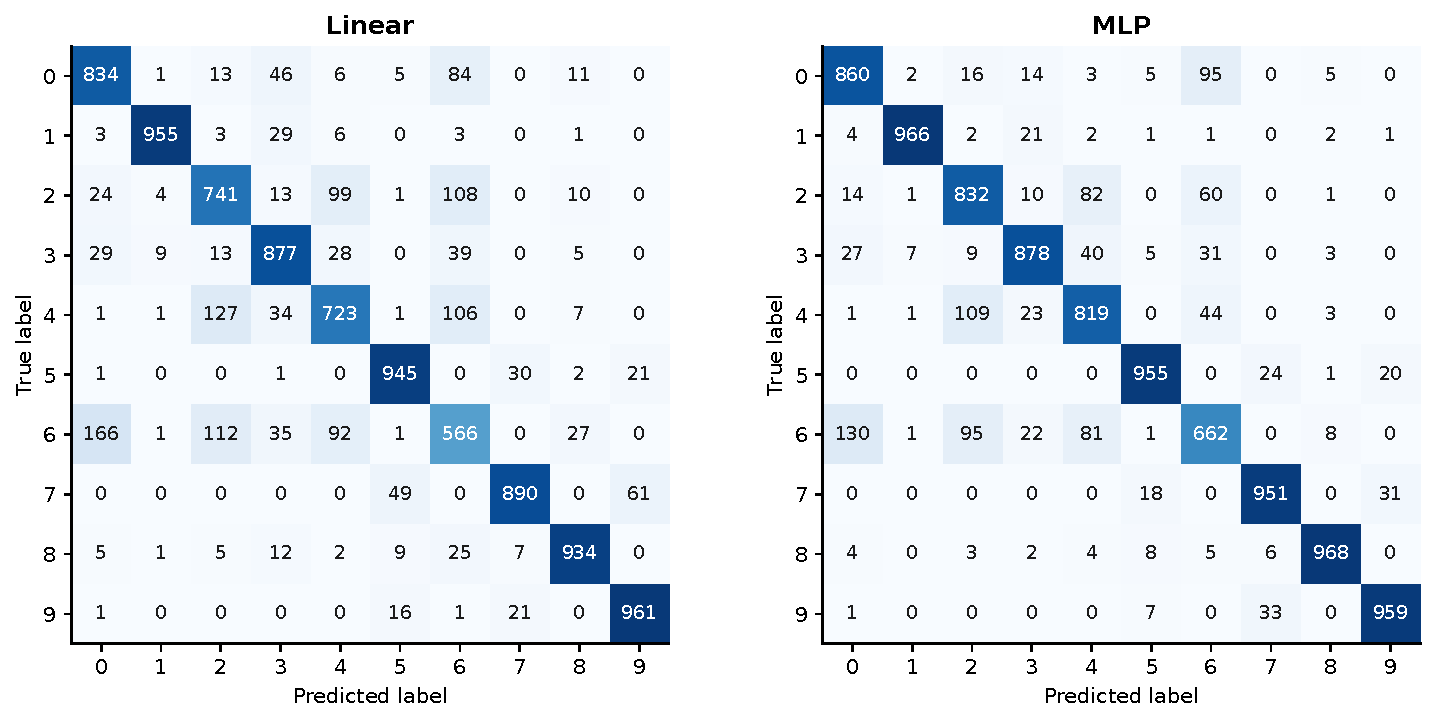
\includegraphics[width=\linewidth]{baseline_confusions.pdf}
\caption{Official-test confusion matrices for the Linear and MLP baselines.}
\end{figure}

\begin{figure}[H]\centering
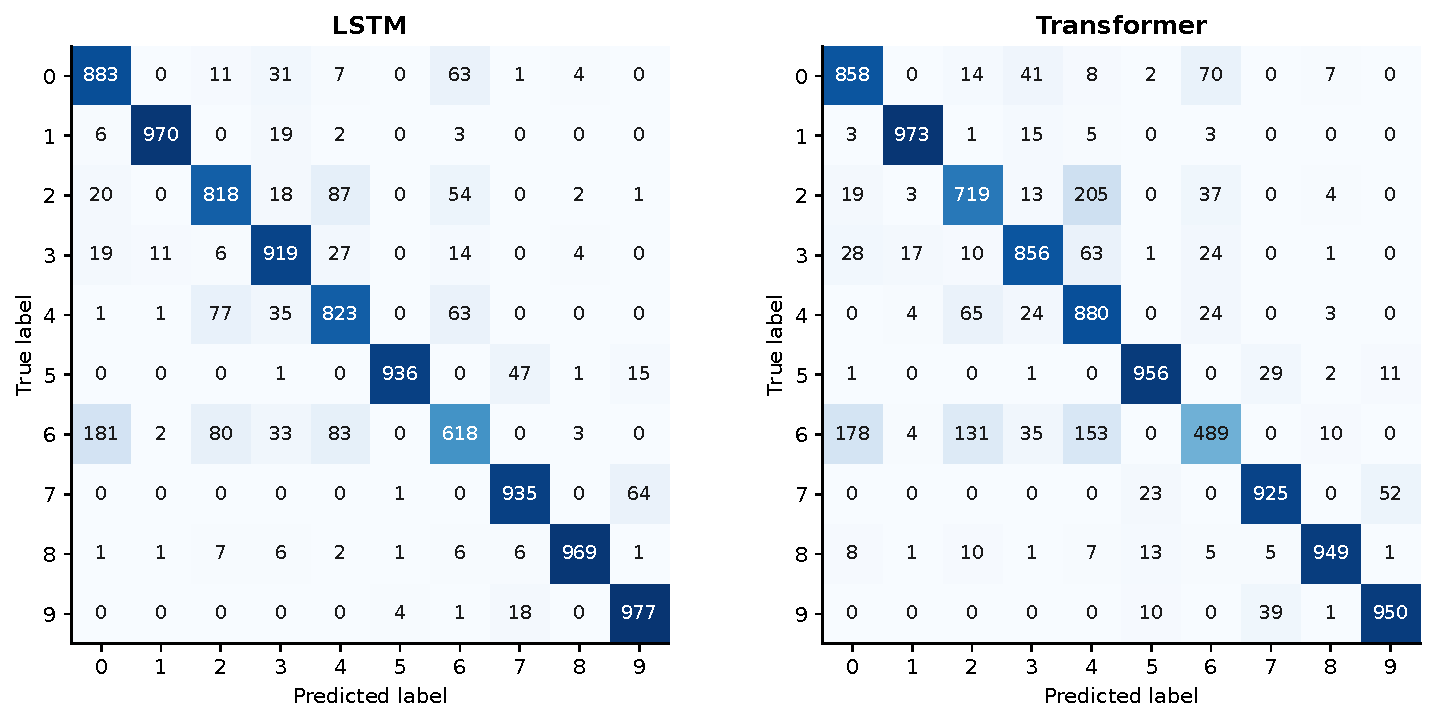
\includegraphics[width=\linewidth]{sequence_confusions.pdf}
\caption{Official-test confusion matrices for the row LSTM and patch Transformer.}
\end{figure}

\small
Labels: 0 T-shirt/top; 1 Trouser; 2 Pullover; 3 Dress; 4 Coat;
5 Sandal; 6 Shirt; 7 Sneaker; 8 Bag; 9 Ankle boot.
\normalsize

\clearpage
\section{Reproducibility and Evidence}
\small
\subsection{Environment and saved files}
The CUDA training and test-evaluation records identify Windows 11,
Python 3.12.10, PyTorch 2.9.1+cu128, torchvision 0.24.1+cu128,
NumPy 2.2.6 and scikit-learn 1.7.2. The GPU is an NVIDIA GeForce
GTX 1660 SUPER with 6 GiB of memory. Linear and MLP computational costs now
come from separate CUDA training and test runs; the original selected
checkpoints remain the source of classification scores and error analysis.

From the repository's \texttt{A1} folder, the principal files are:
\begin{table}[H]\centering\small
\caption{Implementation and experiment evidence.}
\begin{tabularx}{\linewidth}{p{.46\linewidth}X}\toprule
Path & Role\\\midrule
\texttt{a1/data.py} & Split, normalization and input arrangements.\\
\texttt{a1/models.py} & Definitions of all five classifiers.\\
\texttt{a1/train.py} & Training loop and checkpoint selection.\\
\texttt{a1/evaluate.py} & Test evaluation, predictions and timing.\\
\texttt{split\_cache.json} & Fixed indices, hashes and normalization values.\\
\texttt{runs/m1/linear}, \texttt{runs/m1/mlp} & Baseline training and test artifacts.\\
\texttt{runs/cuda\_baselines/linear}, \texttt{mlp} & Separate CUDA baseline cost measurements.\\
\texttt{runs/m2/cnn}, \texttt{lstm}, \texttt{transformer} & Three model directories under \texttt{runs/m2}.\\
\texttt{report/data/eda\_metrics.json} & Training-data statistics and integrity checks.\\\bottomrule
\end{tabularx}
\end{table}

Each run stores a checkpoint, epoch history, training and test summaries,
prediction CSV, confusion matrix and verification record. The test summary's
checkpoint SHA-256 associates its metrics with the exact saved weights.

\subsection{Commands to reproduce the experiment}
Create a Python 3.12 environment and install
\texttt{requirements-windows.txt} on the CUDA reference platform. For example,
run the following from \texttt{A1} in PowerShell:
\begingroup\footnotesize
\begin{verbatim}
py -3.12 -m venv .venv
.\.venv\Scripts\python.exe -m pip install -r requirements-windows.txt
$env:CUBLAS_WORKSPACE_CONFIG = ':4096:8'
.\.venv\Scripts\python.exe -m unittest discover -s tests -v
.\.venv\Scripts\python.exe -m a1.train --model cnn --config configs/cnn.json
.\.venv\Scripts\python.exe -m a1.evaluate --checkpoint runs/m2/cnn/best.pt
.\.venv\Scripts\python.exe tests/verify_run.py --model cnn
\end{verbatim}
\endgroup
Linear and MLP use \texttt{configs/m1.json}; LSTM and Transformer use
\texttt{configs/lstm.json} and \texttt{configs/transformer.json}.
Change the model name and checkpoint directory accordingly.
To reproduce the baseline CUDA cost repetitions without replacing the original
run files, execute the following from \texttt{A1}:
\begin{verbatim}
.\.venv\Scripts\python.exe -m a1.cuda_baselines
\end{verbatim}
This uses \texttt{configs/m1\_cuda.json}, which explicitly requires CUDA and
writes to \texttt{runs/cuda\_baselines}. It trains both baselines, evaluates
their selected checkpoints on CUDA and verifies all saved test predictions.

\subsection{Checks performed for this report}
Report checks recompute metrics and confusion counts for all 50,000 original
test predictions and verify checkpoint selection, normalization, data hashes
and file digests.

Both new CUDA baseline checkpoints pass validation/test metric recomputation,
verification of all 20,000 saved predictions and CPU/CUDA agreement on 128
images per model. Records accompany the checkpoints. Losses and timings use
saved summaries; report evidence and document checks are in \texttt{qa}.

\end{document}
